\documentclass[11pt]{article}

\usepackage[utf8]{inputenc}
\usepackage[T1]{fontenc}
\usepackage{amsmath,amssymb,amsthm}
\usepackage{booktabs}
\usepackage{tikz}
\usepackage[margin=1.15in]{geometry}
\usepackage[hidelinks]{hyperref}

\newtheorem{theorem}{Theorem}
\newtheorem{proposition}[theorem]{Proposition}
\newtheorem{lemma}[theorem]{Lemma}
\theoremstyle{definition}
\newtheorem{definition}{Definition}
\newtheorem{example}{Example}
\theoremstyle{remark}
\newtheorem{remark}{Remark}

\DeclareMathOperator{\E}{\mathbb{E}}
\DeclareMathOperator{\Prob}{\mathbb{P}}
\DeclareMathOperator{\Var}{Var}
\DeclareMathOperator{\Cov}{Cov}
\newcommand{\Pool}{X}
\newcommand{\Luck}{\Lambda}

\title{Measuring skill and luck in feedback-guessing games:\\
a normalised expected-pool skill score and\\
a mid-distribution luck score}
\author{The Lexodle project}
\date{Working draft, \today}

\begin{document}
\maketitle

\begin{abstract}
In a word-guessing game with colour feedback (Wordle and its relatives) a player
can ask two different questions about a guess: was it a \emph{good} guess, and
was the outcome \emph{lucky}? We give each a definition that depends only on what
the player could know. A guess splits the words still possible into the groups
that give the same feedback; the answer, being one of those words, lands in one
group, whose size we call the \emph{pool}. The \emph{skill} of a guess is how far
the expected pool falls, on a logarithmic scale, between ``no split at all'' and
the best split any real guess achieves, a number from $0$ to $100$. The \emph{luck} of an outcome is the
chance of landing in a bigger pool less the chance of landing in a smaller one,
a number strictly between $-100$ and $100$. We prove that luck is a
mid-distribution transform of the pool, that it has mean exactly zero for every
guess, that over a whole game its increments are martingale differences and so
are uncorrelated with the skill of any guess and with each other, and we show
that the two more obvious luck definitions fail: scaling by the expected pool is
unbounded below and scaling both sides by the extremes is biased. We extend the
definitions to games with several boards (a guess shared by four words at once, or
played in turn), describe an exact algorithm, and report experiments on a real
English word list: the best first guess leaves $114.4$ of $4{,}994$ words on
average, a familiar opening such as \textsc{crane} scores $81.6$ (and $97.6$ on a linear scale that
crowds most openings near the top), and a plausible
bound on the best conceivable split, built from the number of feedback patterns,
turns out to be too loose to be useful. We list open problems.
\end{abstract}

\section{Introduction}

In Wordle-like games the player guesses a word and is told, letter by letter,
whether it is in the right place, elsewhere in the word, or absent. Two
questions come naturally after a game, and a player who wants to improve needs
them kept apart. \emph{Skill}: given what was known when the guess was made, how
good was it? \emph{Luck}: given the guess, how fortunate was the feedback that
came back? A guess can be excellent and unlucky, or poor and lucky, and a score
that mixes the two teaches the wrong lesson.

The standard analyses of the game are about \emph{playing} it well. Entropy-based
solvers pick the guess that maximises the expected information in the feedback
\cite{shannon1948,sanderson2022}, in the tradition of the solvers of the code
game Mastermind \cite{knuth1977,kooi2005}; exact methods find optimal strategies
for the original word list \cite{bertsimas2022}, while for generalised word lists
deciding whether a win within a given number of guesses can be guaranteed is
NP-hard \cite{lokshtanov2022}. Newspaper-hosted
review tools report a ``skill'' and a ``luck'' for each guess \cite{nyt2022}, but
to our knowledge their exact formulae are not published. Here we are not asking
how to play. We ask what number should be shown to a player after the game, and
we want that number to have properties a player (and a statistician) can rely on.
Our requirements are:

\begin{enumerate}
\item[(R1)] \textbf{Knowledge only.} Neither score may depend on the answer except
through what the player saw. Two players with the same history and the same guess
get the same skill.
\item[(R2)] \textbf{Bounded and anchored.} Skill runs from $0$ (the guess tells
you nothing) to $100$ (as good as any real guess could be). Luck is symmetric about
$0$ and bounded.
\item[(R3)] \textbf{Fair luck.} Luck should be zero on average, and uncorrelated
with skill, so that it measures fortune and not quality.
\item[(R4)] \textbf{One picture.} Both scores should be readable from a single
plot of the outcomes the guess could have had.
\end{enumerate}

Section~\ref{sec:setting} fixes the setting. Section~\ref{sec:skill} defines skill
and Section~\ref{sec:luck} luck, with the theorems. Section~\ref{sec:multi}
extends both to several boards, Section~\ref{sec:computation} gives the algorithm,
Section~\ref{sec:experiments} the experiments, and Section~\ref{sec:open} lists what
we could not settle. All computations are reproducible from the scripts in
\texttt{docs/paper/experiments} and the implementation in the app
(Section~\ref{sec:repro}).

\section{Setting}\label{sec:setting}

Let $\Omega$ be the finite set of words that are \emph{still possible answers}
given everything the player has seen, $N=|\Omega|\ge 1$, and let $\mathcal G$ be
the finite set of admissible guesses (every real word). We assume $\Omega\subseteq
\mathcal G$: any possible answer may be guessed. Let $\Phi$ be the set of feedback
patterns, here $\{\text{grey},\text{yellow},\text{green}\}^n$ for words of $n$
letters, and $f\colon\mathcal G\times\Omega\to\Phi$ the feedback function. Two
facts about $f$ are used: it is computable, and $f(g,w)$ is all green only when
$g=w$.

\begin{definition}[Prior]
The answer $A$ is uniform on $\Omega$ (assumption (U)). More precisely, given the
whole history of guesses and feedback, $A$ is uniform on the words consistent with
it.
\end{definition}

Assumption (U) is the player's view: a player who does not know how the game
chose its answer cannot weigh the candidates, so each possible word counts the
same. (If the game draws answers by frequency the true prior differs; see
Section~\ref{sec:open}.)

A guess $g\in\mathcal G$ partitions $\Omega$ into the nonempty classes
$C_\varphi=\{w\in\Omega: f(g,w)=\varphi\}$, with sizes $s_1,\dots,s_k$ and
$\sum_i s_i=N$. The answer lands in one class; write $\Pool_g=|C_{f(g,A)}|$ for its
size, the \emph{pool}: the number of words still possible after the guess. If
$m_x$ is the number of classes of size $x$ then
\begin{equation}\label{eq:pool-law}
\Prob(\Pool_g=x)=\frac{x\,m_x}{N}.
\end{equation}
A big class is landed in more often, which is why pools are size-biased.

\section{Skill: the normalised expected pool}\label{sec:skill}

\begin{definition}[Expected pool]
$E(g)=\E[\Pool_g]=\dfrac1N\sum_{i=1}^k s_i^2$.
\end{definition}

\begin{definition}[Best real guess and skill]
$E^\ast=E^\ast(\Omega,\mathcal G)=\min_{g\in\mathcal G}E(g)$. For $N\ge2$ the
\emph{skill} of $g\in\mathcal G$ is
\[
S(g)=\frac{\ln\bigl(N/E(g)\bigr)}{\ln\bigl(N/E^\ast\bigr)}\in[0,1],
\]
and reported as a percentage. For $N=1$ we set $S(g)=1$ if $g$ is the remaining
word and $S(g)=0$ otherwise.
\end{definition}

The logarithm is deliberate. A guess cuts the candidates by a \emph{factor}, and a
guess that leaves $10\%$ of the words is a real step behind one that leaves $1\%$;
on a linear scale they would score $90$ and $99$ and nearly every sensible guess would
sit close to $100$ (Section~\ref{sec:experiments}). The linear version
$(N-E)/(N-E^\ast)$, the fraction of the possible reduction of the expected pool, has
the same endpoints and the same ordering of guesses; only the spacing differs.

\begin{lemma}\label{lem:E}
Let the partition of $g$ have $k$ classes. Then
\begin{enumerate}
\item $\max\{1,N/k\}\le E(g)\le N$, with $E(g)=N$ iff $k=1$ and $E(g)=1$ iff $k=N$,
and $E(g)=N/k$ iff all classes have the same size;
\item if the partition of $g'$ is a proper refinement of that of $g$ then
$E(g')<E(g)$.
\end{enumerate}
\end{lemma}
\begin{proof}
(1) Since $1\le s_i\le N$, $E\ge 1$ with equality iff every $s_i=1$, and
$s_i^2\le N s_i$ gives $E\le N$ with equality iff every nonzero $s_i$ equals $N$,
that is $k=1$. By Cauchy--Schwarz, $\sum s_i^2\ge(\sum s_i)^2/k=N^2/k$, with
equality iff the $s_i$ are equal. (2) A class of size $a_1+\dots+a_r$, $r\ge2$,
split into parts $a_j\ge1$ contributes $(\sum a_j)^2>\sum a_j^2$ before the split
and $\sum a_j^2$ after, because the cross terms are positive.
\end{proof}

\begin{proposition}\label{prop:skill}
Let $N\ge2$ and $\Omega\subseteq\mathcal G$. Then $E^\ast<N$, so $S$ is defined, and
\begin{enumerate}
\item $0\le S(g)\le1$ for every $g\in\mathcal G$; $S(g)=1$ iff $E(g)=E^\ast$ (the
split is as even as the best real guess can make it); $S(g)=0$ iff $g$ does not
divide $\Omega$ at all;
\item $S$ is a strictly decreasing function of $E(g)$, affine in $\ln E(g)$: each
halving of the expected pool adds the same $\ln2/\ln(N/E^\ast)$, and if the partition
of $g'$ properly refines that of $g$ then $S(g')>S(g)$;
\item $S(g)$ is a function of $(\Omega,g,\mathcal G)$ alone. In particular it does
not depend on the answer.
\end{enumerate}
\end{proposition}
\begin{proof}
Take $w\in\Omega\subseteq\mathcal G$. Only $w$ itself gives all green against $w$, so
$\{w\}$ is a class of the partition of $w$; as $N\ge2$ the partition is not
trivial, and Lemma~\ref{lem:E} gives $E(w)<N$ and hence $E^\ast<N$, so the
denominator $\ln(N/E^\ast)$ is positive. Part~(1) then follows from
$E^\ast\le E(g)\le N$ (so $0\le\ln(N/E)\le\ln(N/E^\ast)$) and the lemma, (2) from the
formula and Lemma~\ref{lem:E}(2), and (3) because $E(g)$ and $E^\ast$ are computed
from the classes of $\Omega$ alone.
\end{proof}

\begin{remark}[Relation to entropy]
Let $p_i=s_i/N$. Then $\ln(N/E)=-\ln\sum p_i^2=H_2$ is the R\'enyi entropy of
order $2$ of the partition \cite{renyi1961}, the log of the effective number of
equally likely classes in the sense of Simpson and Hill \cite{simpson1949,hill1973}.
So the skill is a ratio of entropies, $S(g)=H_2(g)/\max_{g'}H_2(g')$: the guess's
information as a share of the best real guess's. The Shannon entropy that
entropy-based solvers maximise is $H=-\sum p_i\ln p_i=\ln N-\E[\ln\Pool_g]$
\cite{shannon1948}, the expected log-reduction of the candidate set; by Jensen
$H\ge H_2$. We use $H_2$ because it is a function of $E=\E[\Pool_g]$, the expected
number of words left, which is also what the plot shows (Section~\ref{sec:luck}). Other
orders $\alpha$ of R\'enyi entropy give other scales; we have not studied them.
\end{remark}

\begin{remark}[Why the best \emph{real} guess]
One might normalise by a bound that does not need a search, such as the most even
split into $\min(N,3^n)$ groups, $e=N/\min(N,3^n)$. Section~\ref{sec:experiments}
tests this, and a sharper bound built from the clues, and finds them too loose:
the best real word reaches only about two thirds of the groups the bound allows
when many words are left, and when few are left it rarely separates every word.
A score whose top end cannot be reached is a poor anchor, so $E^\ast$ is the actual
minimum.
\end{remark}

\section{Luck: the chance-weighted percentile of the pool}\label{sec:luck}

Write $q_x=\Prob(\Pool_g=x)=x\,m_x/N$ for the chance of landing in a pool of size $x$.

\begin{definition}[Luck]
For $x$ in the support of $\Pool=\Pool_g$ put
\[
\Luck_g(x)=\Prob(\Pool>x)-\Prob(\Pool<x).
\]
The \emph{luck} of the outcome is $\Luck_g(\Pool_g)$, reported as a percentage.
\end{definition}

So $\Luck_g(x)$ is the chance of landing in a bigger pool less the chance of landing
in a smaller one: negative when you did worse than most outcomes, positive when you
did better, zero in the middle.

\begin{theorem}\label{thm:luck}
Let $\Pool$ have the law \eqref{eq:pool-law} and let $\Luck=\Luck_g$.
\begin{enumerate}
\item (Mid-distribution form.) $\Luck(x)=2\tilde F(x)-1$ where $\tilde F(x)=
\Prob(\Pool>x)+\tfrac12\Prob(\Pool=x)$. Equivalently $\Luck(\Pool)$ is Cliff's
delta between the realised pool and an independent fresh copy \cite{cliff1993}.
\item (Bounded.) $-1<\Luck(x)<1$ for every $x$ in the support, and $\Luck$ is
strictly decreasing in $x$.
\item (Fair.) $\E[\Luck(\Pool)]=0$, for every guess.
\item (Spread.) $\Var\,\Luck(\Pool)=\dfrac{1-\sum_x q_x^3}{3}<\dfrac13$.
\item (Invariance.) $\Luck(x)$ is unchanged if every class size is multiplied by the
same positive factor, and equal pools receive equal luck.
\end{enumerate}
\end{theorem}
\begin{proof}
(1) $\Prob(\Pool<x)=1-\Prob(\Pool>x)-\Prob(\Pool=x)$, so $\Luck(x)=2\Prob(\Pool>x)+
\Prob(\Pool=x)-1=2\tilde F(x)-1$. With $\Pool'$ an independent copy,
$\Luck(x)=\E[\mathbf 1\{\Pool'>x\}-\mathbf 1\{\Pool'<x\}]$, which is Cliff's delta.

(2) $\Prob(\Pool>x)+\Prob(\Pool<x)=1-q_x<1$ and both are non-negative, so
$|\Luck(x)|<1$. If $x<y$ are in the support then $\Prob(\Pool>x)\ge\Prob(\Pool>y)+q_y$
and $\Prob(\Pool<x)\le\Prob(\Pool<y)-q_x$, so $\Luck(x)>\Luck(y)$.

(3) With $\Pool,\Pool'$ independent and identically distributed,
$\E[\Luck(\Pool)]=\Prob(\Pool'>\Pool)-\Prob(\Pool'<\Pool)=0$ by exchangeability.

(4) List the distinct pool sizes in decreasing order, $x_1>\dots>x_r$, with
masses $q_i$ and $c_i=\sum_{j<i}q_j=\Prob(\Pool>x_i)$, so $\tilde F(x_i)=c_i+q_i/2$.
Since $\sum_i[(c_i+q_i)^3-c_i^3]=1$ telescopes,
\[
\sum_i\bigl(3c_i^2q_i+3c_iq_i^2+q_i^3\bigr)=1,\quad\text{so}\quad
\sum_i q_ic_i^2+\sum_i c_iq_i^2=\frac{1-\sum_i q_i^3}{3}.
\]
Then $\E[\tilde F^2]=\sum_i q_i(c_i+q_i/2)^2=\sum_i q_ic_i^2+\sum_i c_iq_i^2+
\tfrac14\sum_i q_i^3=\tfrac13-\tfrac1{12}\sum_i q_i^3$, and by (3) $\E[\tilde F]=
\tfrac12$, so $\Var\tilde F=\tfrac1{12}(1-\sum_i q_i^3)$ and $\Var\Luck=
4\Var\tilde F$.

(5) Multiplying every $s_i$ by $c>0$ multiplies $N$ and every $q_x$-numerator by $c$,
so each $q_x$ is unchanged and so is $\Luck$. Equal pools are the same $x$.
\end{proof}

\begin{remark}
Theorem~\ref{thm:luck} is the sense in which luck is \emph{chance-weighted}. It is a
percentile because it is the mid-distribution transform \cite{lancaster1961,parzen2004}
of the pool, a discrete analogue of the probability integral transform
\cite{rosenblatt1952}; the mid-rank convention gives ties the average position,
which is what makes the mean exactly zero. Columns of a plot as wide as their chance
make the horizontal middle the median outcome, and $\Luck$ is the centre of the
column of the landed pool measured from that middle (Figure~\ref{fig:example}).
\end{remark}

\subsection{Luck is uncorrelated with skill}

Let $\mathcal F_{t-1}$ be the history before the $t$-th guess and suppose the
player's guess $g_t$ is a function of $\mathcal F_{t-1}$ and possibly of
independent randomness. Let $S_t$ and $\Luck_t=\Luck_{g_t}(\Pool_{g_t})$ be the
skill and luck of that guess.

\begin{theorem}\label{thm:martingale}
Under (U), $\E[\Luck_t\mid\mathcal F_{t-1}]=0$. Consequently $\E\Luck_t=0$,
$\Cov(\Luck_t,S_s)=0$ for every $s\le t$, and $\Cov(\Luck_s,\Luck_t)=0$ for
$s\ne t$; and the cumulative luck $\sum_{s\le t}\Luck_s$ is a martingale.
\end{theorem}
\begin{proof}
Given $\mathcal F_{t-1}$ the answer is uniform on the consistent words $\Omega_t$ and
$g_t$ is fixed, so Theorem~\ref{thm:luck}(3) applies conditionally. The skill $S_s$ for
$s\le t$ and the luck $\Luck_s$ for $s<t$ are $\mathcal F_{t-1}$-measurable, hence
$\Cov(\Luck_t,S_s)=\E[S_s\E[\Luck_t\mid\mathcal F_{t-1}]]-\E S_s\,\E\Luck_t=0$, and
likewise for $\Luck_s\Luck_t$.
\end{proof}

Theorem~\ref{thm:martingale} is (R3): however well or badly someone plays, their luck
averages zero and is not predicted by how skilfully they played so far.

\subsection{The obvious alternatives fail}\label{sec:alternatives}

Two natural definitions scale the gap between the landed pool $a$ and the expected
pool $E$.

\begin{proposition}\label{prop:alternatives}
Let $E>1$.
\begin{enumerate}
\item The expectation-scaled luck $\Luck^{\exp}(a)=(E-a)/(E-1)$ has mean zero but is
not bounded below: for the partition of $N$ words into one pair and $N-2$ singletons,
landing in the pair gives $-(N-2)/2$.
\item The rescaled luck, $\Luck^{\mathrm{res}}(a)=(E-a)/(E-1)$ for $a\le E$ and
$(E-a)/(a_{\max}-E)$ for $a>E$, lies in $[-1,1]$, but its mean is
$\kappa\bigl(\tfrac1{E-1}-\tfrac1{a_{\max}-E}\bigr)$ with $\kappa=\E[(E-\Pool)^+]$,
which is nonzero unless $a_{\max}-E=E-1$. For the partition $\{3,1\}$ it is $-\tfrac12$.
\end{enumerate}
\end{proposition}
\begin{proof}
(1) $\E\Luck^{\exp}=(E-\E\Pool)/(E-1)=0$. For the pair and $N-2$ singletons, $E=(N+2)/N$,
so $E-1=2/N$ and $E-2=-(N-2)/N$, and the ratio is $-(N-2)/2$.
(2) Since $\E[\Pool-E]=0$, $\E[(E-\Pool)^+]=\E[(\Pool-E)^+]=\kappa$; the positive part
of $\Luck^{\mathrm{res}}$ is scaled by $1/(E-1)$ and the negative part by
$1/(a_{\max}-E)$. For $\{3,1\}$: $N=4$, $E=\tfrac52$, $a_{\max}=3$; landing in the
$3$ (chance $\tfrac34$) gives $-1$ and landing in the $1$ gives $+1$, mean $-\tfrac12$.
\end{proof}

The first is unbounded, violating (R2); the second is bounded but biased, so it mixes
the quality of the guess into luck, violating (R3): Section~\ref{sec:experiments}
gives means from $+19\%$ to $-60\%$ on real positions. The chance-weighted luck is
bounded and fair at once. It is also the only one of the three that is defined by
\emph{ranking} outcomes, which is what a plot of the outcomes shows.

\subsection{The last try}

On the last allowed guess nothing is left to learn; only a word that fits can win.
Say $n$ words fit the clues. A guess that is one of them wins with chance $1/n$; a
guess that is not one of them cannot win and wins with chance $0$.

\begin{proposition}\label{prop:last}
Let $Y=\mathbf 1\{\text{win}\}$ and $\pi=\Prob(\text{win})\in\{1/n,0\}$. The last-try
luck $\Luck=Y-\pi$ has mean zero for every guess, takes the values $1-\pi$ and $-\pi$,
and lies in $(-1,1)$ for $n\ge2$; it is $0$ for a guess that cannot win, whose loss is
a matter of skill. With three words fitting, a hit is $+67\%$ and a miss $-33\%$.
\end{proposition}
\begin{proof}
$\E Y=\pi$, so $\E[Y-\pi]=0$; the range follows from $0\le\pi\le\tfrac12$ for $n\ge2$.
\end{proof}

\begin{figure}[t]
\centering
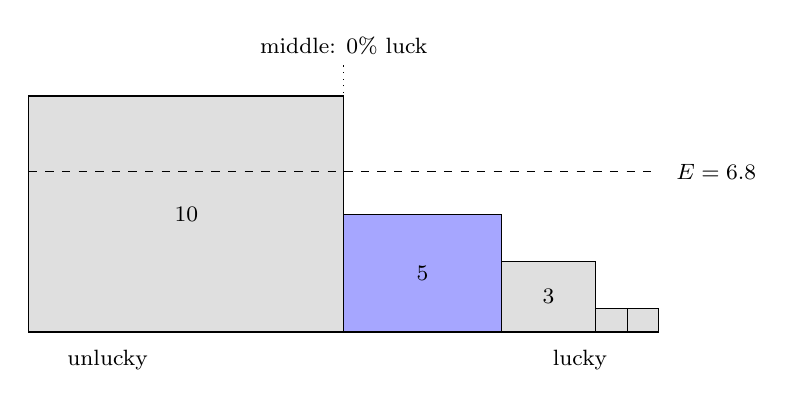
\begin{tikzpicture}[x=1cm,y=1cm]
% N = 20 words, groups of 10, 5, 3, 1, 1; widths = chance, heights = pool size
\draw[fill=gray!25] (0,0) rectangle (4,3.0);
\draw[fill=blue!35] (4,0) rectangle (6,1.5);
\draw[fill=gray!25] (6,0) rectangle (7.2,0.9);
\draw[fill=gray!25] (7.2,0) rectangle (7.6,0.3);
\draw[fill=gray!25] (7.6,0) rectangle (8,0.3);
\draw[thick] (0,0) -- (8,0);
\draw[dashed] (0,2.04) -- (8,2.04);
\draw[dotted] (4,0) -- (4,3.4);
\node[anchor=west,font=\footnotesize] at (8.1,2.04) {$E=6.8$};
\node[anchor=south,font=\footnotesize] at (4,3.4) {middle: $0\%$ luck};
\node[font=\footnotesize] at (2,1.5) {10};
\node[font=\footnotesize] at (5,0.75) {5};
\node[font=\footnotesize] at (6.6,0.45) {3};
\node[anchor=north,font=\footnotesize] at (1,-0.1) {unlucky};
\node[anchor=north,font=\footnotesize] at (7,-0.1) {lucky};
\end{tikzpicture}
\caption{The guess of Example~\ref{ex:twenty}: twenty words split into groups of
$10,5,3,1,1$. Each column is as wide as its chance and as tall as its pool; the
dashed line is the expected pool $E=6.8$. Landing in the group of $5$ (shaded) has
luck $+25\%$: the chance of a bigger pool ($10/20$) less that of a smaller one
($5/20$).}
\label{fig:example}
\end{figure}

\begin{example}\label{ex:twenty}
Twenty words are split into groups of $10,5,3,1,1$. Then $E=(100+25+9+1+1)/20=6.8$,
and if no real guess does better than singletons ($E^\ast=1$) the skill is
$\ln(20/6.8)/\ln20=36.0\%$ (on a linear scale it would be $(20-6.8)/19=69.5\%$). Luck by landing: in the $10$, $\Luck=0-\tfrac{10}{20}=-50\%$;
in the $5$, $\tfrac{10}{20}-\tfrac{5}{20}=+25\%$; in the $3$, $\tfrac{15}{20}-
\tfrac2{20}=+65\%$; in a $1$, $\tfrac{18}{20}-0=+90\%$ (the two singletons tie, and
neither counts against the other). The mean, weighting each by its chance, is
$\tfrac{10}{20}(-.5)+\tfrac5{20}(.25)+\tfrac3{20}(.65)+\tfrac2{20}(.9)=0$.
\end{example}

\section{Several boards}\label{sec:multi}

Variants of the game hide several words at once. We treat two. In a \emph{quartet}
one guess is played on every unsolved board simultaneously; in a \emph{relay race}
the boards are played in turn, and every earlier guess is applied to a board when it
opens (so a guess also works for the boards still to come).

Let a guess $g$ be made for the live boards $b=1,\dots,B$ with possible sets
$\Omega_b$ of sizes $N_b$, with skill $S_b$ and luck $\Luck_b$ computed as above on
each board against that board's own best real guess $E_b^\ast$ (so each is a function
of that board's candidates alone). Define the weights $w_b=\log_2\max\{N_b,2\}$,
which depend only on the history, and
\[
S=\frac{\sum_b w_bS_b}{\sum_b w_b},\qquad
\Luck=\frac{\sum_b w_b\Luck_b}{\sum_b w_b}.
\]

\begin{proposition}\label{prop:multi}
$S\in[0,1]$ and $-1<\Luck<1$. If, given the history, each answer is uniform on its
board's candidates (no independence between boards is assumed), then
$\E[\Luck\mid\mathcal F_{t-1}]=0$, and Theorem~\ref{thm:martingale} holds for the
combined luck.
\end{proposition}
\begin{proof}
Convex combinations of numbers in $[0,1]$ and in $(-1,1)$ stay there. The weights are
$\mathcal F_{t-1}$-measurable, so by linearity of conditional expectation
$\E[\Luck\mid\mathcal F_{t-1}]=\sum_b w_b\E[\Luck_b\mid\mathcal F_{t-1}]/\sum w_b=0$ by
Theorem~\ref{thm:luck}(3) applied to each board. The rest of
Theorem~\ref{thm:martingale}'s proof uses only this.
\end{proof}

\begin{remark}[The weights]
The weight $\log_2N_b$ is the number of bits still to be found on board $b$, so a board
with a thousand words left counts about ten times a board with two. A board with one
word left, which only has to be played out, counts as one bit, so playing that word
is rewarded and missing it is not free; its skill is $1$ if the guess is that word
and $0$ otherwise. Uniform weights would let a nearly solved board dominate the
guess's score; this is a design choice we do not claim is canonical.
\end{remark}

\begin{remark}[Head start]
In a relay race a guess made on the active board narrows the boards not yet open. We do
not score that credit. We report it instead: the \emph{head start} of a board is the
number of words still possible on it at the moment it opens, with every earlier guess
applied, against the size of the whole list. A guess made earlier can even solve a
board the moment it opens. How to assign this credit to the earlier guesses is open.
\end{remark}

\section{Computation}\label{sec:computation}

Feedback for a guess of $n$ letters is packed into one integer in $\{0,\dots,3^n-1\}$.
For a guess $g$, the class sizes of $\Omega$ are counted in an array indexed by
pattern, which is reset by revisiting only the patterns touched, so $E(g)$ costs one
pass of $O(nN)$ and no allocation. The skill of a guess needs $E^\ast=\min_gE(g)$,
a scan of all $|\mathcal G|$ real guesses: $O(n\,N|\mathcal G|)$, about $1.2\times10^8$
elementary operations for the first guess in an English list of five-letter words
($N=|\mathcal G|=4{,}994$) and far fewer afterwards as $N$ falls. The scan also yields
the skill of every guess, so the ranking of the player's guess among all real guesses
comes free. For several boards, boards that share the very same list of candidates
(all of them at the start) are scored once. A truncated scan gives an $E^\ast$ that is
too large, so a skill that is too high; the app scans every real guess.

Luck needs only the class sizes of the player's guess: sort the distinct sizes and
accumulate the masses above and below, $O(k\log k)$ for $k$ classes.

\section{Experiments}\label{sec:experiments}

All figures come from the English five-letter list of the app ($N=4{,}994$, every
word a legal guess and a possible answer), computed by the scripts in
\texttt{docs/paper/experiments} (results in the \texttt{results} directory).

\subsection{First guesses}

Table~\ref{tab:first} gives $E$, the number of groups, the largest group and the
skill of some openings, with the linear skill $(N-E)/(N-E^\ast)$ for comparison. The
best first guess, \textsc{tares}, leaves $114.4$ words on average.

\begin{table}[t]
\centering
\begin{tabular}{lrrrrrr}
\toprule
guess & rank & $E$ & groups & largest & skill & linear\\
\midrule
tares & 1 & 114.4 & 184 & 350 & 100.0 & 100.0\\
slate & 24 & 138.0 & 174 & 355 & 95.0 & 99.5\\
trace & 534 & 219.8 & 155 & 625 & 82.7 & 97.8\\
crane & 628 & 229.3 & 155 & 641 & 81.6 & 97.6\\
abbey & 3786 & 550.9 & 78 & 1069 & 58.4 & 91.1\\
queue & 4907 & 1218.5 & 40 & 2063 & 37.4 & 77.4\\
mamma & 4973 & 1681.5 & 49 & 2693 & 28.8 & 67.9\\
xxxix & 4994 & 2828.0 & 21 & 3598 & 15.1 & 44.4\\
\bottomrule
\end{tabular}
\caption{First guesses, English five-letter words, ranked by $E$ among all $4{,}994$.}
\label{tab:first}
\end{table}

The linear score compresses the top, which is why the logarithmic one is used. Over all
$4{,}994$ words as first guesses the median linear skill is $94.3$ and $81.1\%$ score above
$90$ ($42.7\%$ above $95$); on the logarithmic scale the median is $67.4$ and only $2.7\%$
score above $90$ ($0.5\%$ above $95$). Linear skill is honest as the fraction of the
possible reduction in expected words left but, early in a game, nearly every sensible guess
is close to $100$ and the number says little.

\subsection{Three definitions of luck}

Table~\ref{tab:luck} shows the luck of landing in the largest pool and the mean luck over
all answers for each definition of Section~\ref{sec:alternatives}. The expectation-scaled
luck reaches $-208\%$ for the largest pool of \textsc{tares}; the rescaled luck is
confined to $[-100,100]$ but averages from $+18.8\%$ to $-21.5\%$ over answers on first
guesses, and $-60\%$ in a late position (five words left); the chance-weighted luck
averages $0$ to the precision shown in every case.

\begin{table}[t]
\centering
\begin{tabular}{lrrrrrrr}
\toprule
 & & & \multicolumn{3}{c}{largest pool} & \multicolumn{2}{c}{mean over answers}\\
\cmidrule(lr){4-6}\cmidrule(lr){7-8}
guess & $E$ & largest & exp. & resc. & chance & resc. & chance\\
\midrule
tares & 114.4 & 350 & $-208\%$ & $-100\%$ & $-93\%$ & $+18.8\%$ & $0.0\%$\\
crane & 229.3 & 641 & $-180\%$ & $-100\%$ & $-87\%$ & $+18.1\%$ & $0.0\%$\\
abbey & 550.9 & 1069 & $-94\%$ & $-100\%$ & $-79\%$ & $-1.8\%$ & $0.0\%$\\
queue & 1218.5 & 2063 & $-69\%$ & $-100\%$ & $-59\%$ & $-12.7\%$ & $0.0\%$\\
mamma & 1681.5 & 2693 & $-60\%$ & $-100\%$ & $-46\%$ & $-21.5\%$ & $0.0\%$\\
\bottomrule
\end{tabular}
\caption{Luck of landing in the largest pool (expectation-scaled, rescaled,
chance-weighted) and mean luck over all answers (the expectation-scaled mean is zero
by construction). Words as in Table~\ref{tab:first}.}
\label{tab:luck}
\end{table}

For \textsc{crane}, landing in the $641$-word pool (chance $12.8\%$) is $-87\%$, in a $328$-word
pool $-47\%$, in a $23$-word pool $+71\%$, and in a single word $+99\%$. Landing in
a pair among $N-2$ singletons is $-(N-2)/N$ chance-weighted, against $-(N-2)/2$
expectation-scaled: $-98\%$ against $-4{,}900\%$ at $N=100$.

\subsection{Simulated players}

\texttt{play\_skill.py} plays $60$ games each for a strong player (a good opener, then
always the consistent word that leaves the fewest words) and a casual one (a random common
opener, then a random consistent word), answers uniform on the list, scoring every guess on
the logarithmic scale. Per guess the strong player's median is $100$ (mean $90$) and the
casual player's $74$ (mean $74$). In won games the strong player has every guess above $80$
in $64\%$ and above $90$ in $27\%$; the casual player in $0\%$ for both. The scale thus
separates the two kinds of play with room at the top, where on the linear scale nearly every
guess of either would score above $90$.

\subsection{The game's own answer draw}

Luck is fair (mean zero) when each possible word is equally likely to be the answer. The
game instead draws the answer by word frequency. \texttt{prior\_bias.py} measures the
mean luck of a first guess under that draw: it is $+10.2\%$ for \textsc{tares}, $+10.6\%$
for \textsc{crane}, $+7.6\%$ for \textsc{slate} and $-6.4\%$ and $-8.2\%$ for the weak
openings \textsc{abbey} and \textsc{mamma} (restricting the draw to the $500$ most common
words moves these by about a point). So under the real draw luck is slightly positive for
good openings and negative for poor ones: the common words the game likes to choose
tend to fall in small groups of strong guesses and large groups of weak ones. Under the
uniform assumption of the player's view the means are zero to machine precision
(Table~\ref{tab:luck}); the discrepancy is the subject of the first open problem.

\subsection{A bound on the best conceivable split: a negative result}

We tested three bounds on the number of groups: the naive $\min(N,3^n)$; a bound
$B$ that counts $2$ outcomes at positions the clues fix and $3$ elsewhere; and a bound
$C$ that takes, over all real guess words, the product over letters of how many of
green/yellow/grey that letter could show against the words still possible. On $14$
simulated games ($40$ positions after $0$, $1$ or $2$ guesses) $B$ and $C$ equal the
naive bound in every position: the clues never reduced the capacity below
$\min(N,243)$. The bounds are far above what real words reach: where $N>243$ the best
scanned real guess made about $63\%$ of the groups allowed, and where $N\le243$ a real
guess separated every word in only $3$ of $20$ positions. Bound $C$ is not even valid for
repeated letters ($7$ of $109{,}782$ guesses exceeded it, all with a repeated letter).
So the bound gives no reachable ``best'' and we normalise by the best real guess.

\subsection{Checking the theorems numerically}

\texttt{verify\_theorems.py} checks Theorems~\ref{thm:luck} and~\ref{thm:martingale}
and Proposition~\ref{prop:alternatives} independently of the app. On $20{,}000$ random
partitions luck lies strictly in $(-1,1)$, is strictly monotone in the pool, is unchanged by
scaling the classes, has $|\text{mean}|<2\times10^{-16}$ and has variance equal to
$(1-\sum q^3)/3$ to the same precision. On $1{,}500$ simulated games of four guesses, with
the answer uniform on the list and the player's guesses depending only on the past, the
mean luck of each guess is within sampling error of zero (for example $+0.008$ with
standard deviation $0.57$ on the first guess), and all correlations of a guess's luck with
the skill of any guess so far, and with the luck of earlier guesses, are within four standard
errors of zero (the largest in magnitude is $0.084$ against a tolerance of $0.103$).

\section{Open problems}\label{sec:open}

\begin{enumerate}
\item \textbf{Non-uniform priors.} If answers are drawn by word frequency, replace sizes
by prior masses: $E=\sum_iW_i^2/W$ with $W_i$ the mass of class $i$. Theorems~\ref{thm:luck}
and~\ref{thm:martingale} go through with $p_i=W_i/W$, which would remove the bias of about
$\pm10$ points measured above, but it is unclear whether the ``pool'' being ranked should be
the count of words or the mass, and a player cannot be expected to know the frequencies.
\item \textbf{Lookahead.} Skill is one-step: it scores the split a guess makes now. A
guess can be worse than another by this measure and better over the rest of the game.
Is there a consistent skill that credits lookahead and is still a function of the
player's knowledge alone, perhaps through the expected number of further guesses of an
optimal continuation \cite{bertsimas2022}?
\item \textbf{The scale of skill.} We use the logarithm of the expected pool, the
R\'enyi order-$2$ entropy, because the linear scale packs first guesses near $100$
(Section~\ref{sec:experiments}). Is this the best scale for telling a player how they
did? Other orders of R\'enyi entropy, or a scale calibrated to the number of guesses a
strong player needs, are alternatives, and the choice could be tested against how
strong players rank openings.
\item \textbf{Luck and the structure of a game.} Luck is uncorrelated with skill
(Theorem~\ref{thm:martingale}); is there a natural \emph{normalised} total luck for a game
of several guesses, comparable across games of different length, for example $\sum_t
\Luck_t/\sqrt{\sum_t\Var\Luck_t}$?
\item \textbf{Relay-race credit.} How should the head start of a board, which comes
from earlier guesses, be credited to those guesses?
\item \textbf{Ties.} We use mid-ranks for equal pools. Strict ranks give a luck that is
not mean zero; other tie rules (random, lexicographic) are possible. Is the mid-rank
rule characterised by fairness?
\item \textbf{Hard modes, other feedback.} The results use only that $f$ is a function
into a finite set with all-green exactly at equality; do the bounds and the algorithm
extend to games where later guesses must obey earlier clues, and how does $E^\ast$
change?
\item \textbf{Approximating $E^\ast$.} The exact scan is quadratic in the list. Are
there provable shortcuts, such as a sound lower bound on $E^\ast$ from the letter
statistics of $\Omega$, that make skill cheap on very large lists or scripts with many
more patterns?
\end{enumerate}

\section{Reproducibility}\label{sec:repro}

The app computes these quantities in \texttt{app/lib/logic.dart} (\texttt{scoreGuess},
\texttt{chanceLuck}, \texttt{skillAgainst}, \texttt{analyseGuesses}) and
\texttt{app/lib/multi\_analysis.dart} (\texttt{analyseMulti}); the properties above are
tested in \texttt{app/test/logic\_test.dart}, \texttt{review\_plots\_test.dart} and
\texttt{multi\_analysis\_test.dart}, including bounds, zero mean over $500$ random
partitions and the equality of the plot geometry with the table. The experiments are
\texttt{first\_guess.py}, \texttt{first\_guess\_summary.py},
\texttt{luck\_definitions.py}, \texttt{prior\_bias.py}, \texttt{play\_skill.py},
\texttt{capacity\_bound.py} and \texttt{verify\_theorems.py} in
\texttt{docs/paper/experiments}, sharing \texttt{common.py}; each states its command and
output file.

\begin{thebibliography}{99}

\bibitem{shannon1948} C.~E. Shannon. A mathematical theory of communication.
\emph{Bell System Technical Journal}, 27(3):379--423 and 27(4):623--656, 1948.

\bibitem{knuth1977} D.~E. Knuth. The computer as Master Mind.
\emph{Journal of Recreational Mathematics}, 9(1):1--6, 1976--77.

\bibitem{kooi2005} B.~Kooi. Yet another Mastermind strategy.
\emph{ICGA Journal}, 28(1):13--20, 2005.

\bibitem{bertsimas2022} D.~Bertsimas and A.~Paskov. An exact and interpretable
solution to Wordle. Preprint, 2022.

\bibitem{lokshtanov2022} D.~Lokshtanov and B.~Subercaseaux. Wordle is NP-hard.
In \emph{11th International Conference on Fun with Algorithms (FUN 2022)}, LIPIcs 226,
19:1--19:8, 2022.

\bibitem{sanderson2022} G.~Sanderson. Solving Wordle using information theory.
Video, 3Blue1Brown, 2022.

\bibitem{nyt2022} The New York Times. WordleBot. Online tool, 2022.

\bibitem{simpson1949} E.~H. Simpson. Measurement of diversity. \emph{Nature}, 163:688,
1949.

\bibitem{renyi1961} A.~R\'enyi. On measures of entropy and information. In
\emph{Proceedings of the Fourth Berkeley Symposium on Mathematical Statistics and
Probability}, volume~1, pages 547--561, 1961.

\bibitem{hill1973} M.~O. Hill. Diversity and evenness: a unifying notation and its
consequences. \emph{Ecology}, 54(2):427--432, 1973.

\bibitem{lancaster1961} H.~O. Lancaster. Significance tests in discrete distributions.
\emph{Journal of the American Statistical Association}, 56(294):223--234, 1961.

\bibitem{parzen2004} E.~Parzen. Quantile probability and statistical data modeling.
\emph{Statistical Science}, 19(4):652--662, 2004.

\bibitem{rosenblatt1952} M.~Rosenblatt. Remarks on a multivariate transformation.
\emph{Annals of Mathematical Statistics}, 23(3):470--472, 1952.

\bibitem{cliff1993} N.~Cliff. Dominance statistics: ordinal analyses to answer ordinal
questions. \emph{Psychological Bulletin}, 114(3):494--509, 1993.

\end{thebibliography}

\end{document}
